\documentclass[a4paper,12pt]{article}

% don't forget the document class, generally : \documentclass[a4paper,12pt]{article}

\usepackage[utf8]{inputenc}
\usepackage[french]{babel}
\usepackage{graphicx}
\usepackage{gensymb}
\usepackage{amsmath}
\usepackage{float}
\usepackage{scrextend}
\usepackage{caption} 
\usepackage{siunitx}
\usepackage{enumitem}
\usepackage{amsthm}
\usepackage{fancyhdr}
\usepackage{amssymb}
\usepackage{wrapfig}
\usepackage{geometry}
\usepackage{standalone}
\usepackage{import}
\usepackage[usenames, dvipsnames]{color}

 \usepackage{biblatex} % manages bibliography and references
\addbibresource{sample.bib}


\geometry{hmargin=1in, vmargin=1in}

 \newenvironment{absolutelynopagebreak}
 {\par\nobreak\vfil\penalty0\vfilneg
 \vtop\bgroup}
 {\par\xdef\tpd{\the\prevdepth}\egroup
 \prevdepth=\tpd}
 
 \pagestyle{fancy}                        
\fancyhf{}                               
\fancyhf[HL]{Application des maths}                
\fancyhf[HR]{Géométrie euclidienne}             
\fancyhf[FC]{\thepage/\pageref{Lastpage}}
 
\newtheorem{definition}{Définition}[section]
\newtheorem{theorem}{Théorème}
\newtheorem{corollary}{Corollaire}[theorem]
\newtheorem{lemma}[theorem]{Lemme}
\newtheorem*{hyp}{Hypothèse}
\newtheorem*{concl}{Conclusion}
\newtheorem*{remark}{Remarque}

\captionsetup{format=default,labelformat=simple,labelsep=colon,
justification=justified,font={sf,small},labelfont=bf,
textfont=default} 



\begin{document}

\begin{corollary} \label{cor:mediatrices}
Les médiatrices d'un triangle se croisent en un point unique, le centre du cercle circonscrit du triangle $ABC$.
\end{corollary}
\begin{proof}
Nous considérons un triangle quelconque $ABC$. Nous nommons $I$ l'intersection des médiatrices des côtés $AC$ ($M_{AC}$) et $BC$ ($M_{BC}$).

\begin{hyp}
$I \in M_{AC}$ et $I \in M_{BC}$
\end{hyp}
\begin{concl}
$I \in M_{AB}$ (la médiatrice du côté $AB$) 
\end{concl}

En considérant l'hypothèse et la définition de la médiatrice (définition \ref{def:mediatrice}), nous savons que $IA \equiv IC$ et que $IB \equiv IC$ (on observent deux paires de triangles isométriques). Par conséquent, $IA \equiv IB$. Puisque $I$ est à une distance équivalente de $A$ et de $B$, $I \in M_{AB}$.\\
\begin{figure}[H]
        \centering
        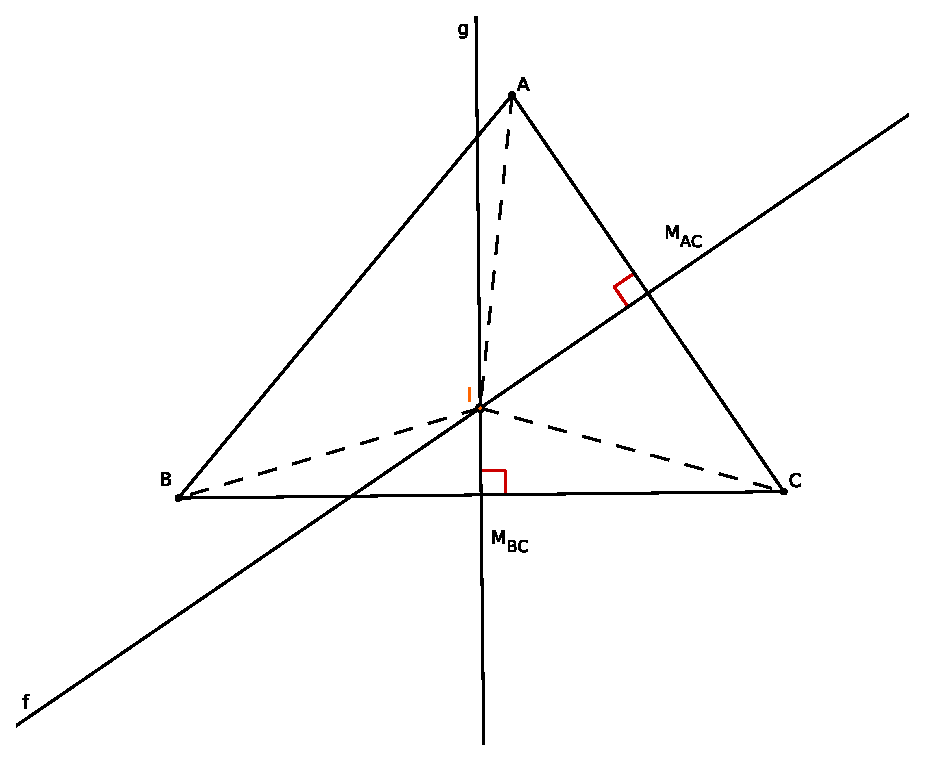
\includegraphics[scale=1]{corMediatrice.eps}
    \end{figure}

De plus, puisque $I$ est le lieu des points équidistants à $A$, $B$ et $C$, c'est aussi le cercle du cercle circonscrit de $\triangle ABC$.
\end{proof}

\end{document}